\documentclass[10pt]{article}

% Pacotes extras necessários
\usepackage{amsmath}
\usepackage[lmargin=0.5in, rmargin=0.5in, tmargin=0.5in, bmargin=0.5in, includehead, includefoot]{geometry}
\usepackage{amsfonts}
\usepackage[utf8]{inputenc}
\usepackage[portuguese]{babel}
\usepackage{graphicx}
\usepackage{fancyhdr}
\usepackage{setspace}
\usepackage{listings}

\graphicspath{ {./images/} }

% Sets para outras partes
\setlength{\parindent}{0pt}
\setstretch{1.5}
\DeclareMathOperator{\sen}{sen}
\DeclareMathOperator{\sinc}{sinc}

%% Facilidades
%% -- Laplace
\newcommand{\Lap}[1]{\mathcal{L}\left\{#1\right\}}

%% -- Negrito em matemáticas
\newcommand{\bm}[1]{\boldsymbol{#1}}


% ------- Estilo do trabalho -------- %
\fancypagestyle{capa}{
    \fancyhf{}
    \renewcommand\headrulewidth{0pt}
}

\pagestyle{fancy}
\fancyhead{}
\fancyhead[L]{\thepage}
\fancyfoot{}
% ----------------------------------- %

% Dados do Grupo
\title{Modelagem de Sistemas Dinâmicos - Trabalho Nº1}
\author{
    Leonardo Soares da Costa Tanaka - DRE: 121067652 \\
    Engenharia de Controle e Automação/UFRJ \\
    Rio de Janeiro, Brasil
}

\date{}

\begin{document}
\maketitle
\thispagestyle{capa}

\section{Introdução}

\quad Considerando um sistema linear invariante no tempo de u(t), saída y(t) e 
função de transferência dada por:

\begin{equation}
    H(s) = \frac{100}{16} \frac{s^2 + 16}{s^2 + 0.2s + 100}
\end{equation}

\quad Com essa função de transferência, é possível obter os zeros e pólos do sistema utilizando a Fórmula de Bhaskara no numerador e denominador da função de transferência.
Os valores dos zeros e pólos do sistema são:
$z_1 = 4j$, $z_2 = -4j$, $p_1 = -0,1 + 9,9995j$ e $p_2 = -0,1 - 9,9995j$.

\begin{equation}
    x = \frac{-b \pm \sqrt{b^2 - 4ac}}{2a}
\end{equation}

\quad Plotando o Diagrama de Bode em Python com o seguinte código:

\begin{figure}[h]
    \centering
    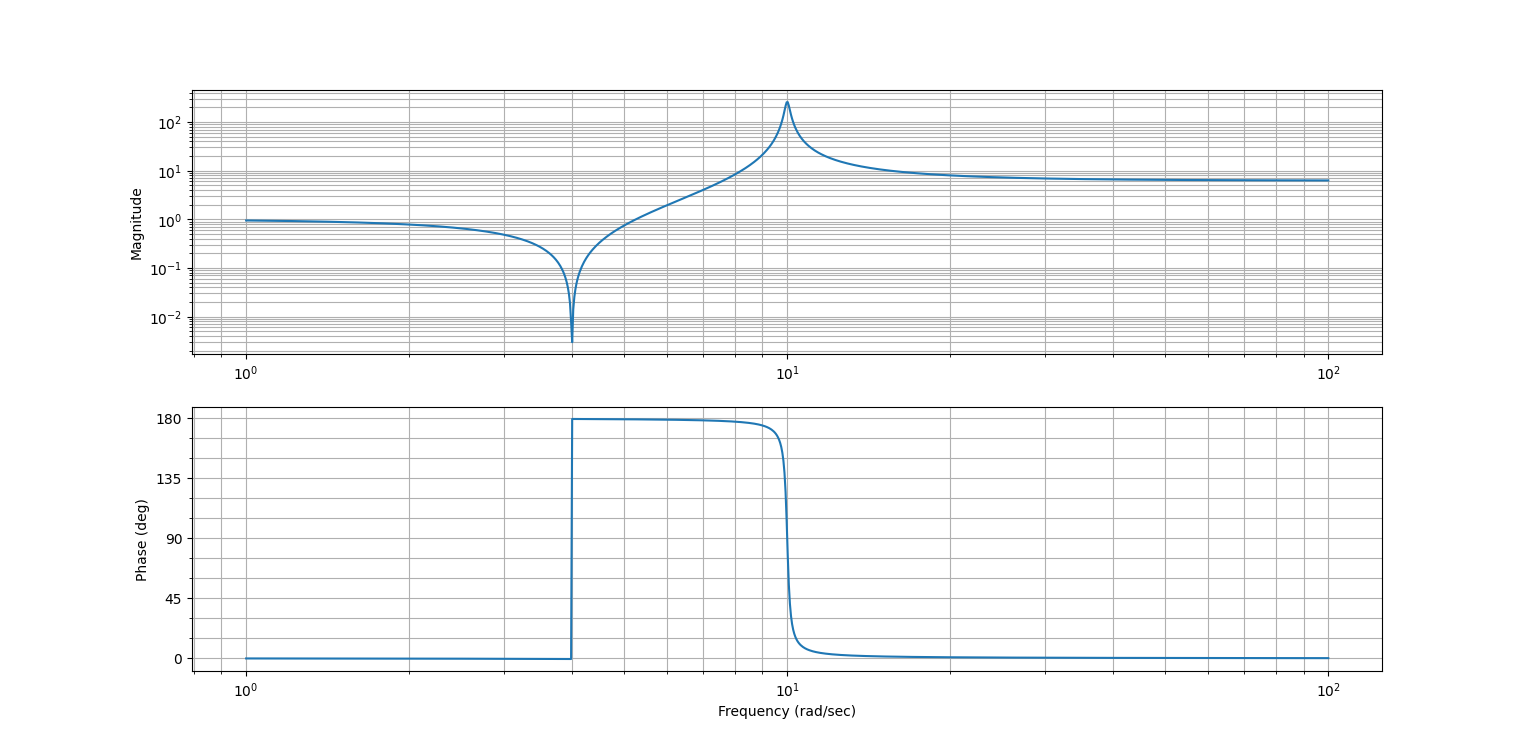
\includegraphics[scale=0.4]{bode.png}
    \caption{Diagrama de Bode}
\end{figure}

\begin{lstlisting}
import control as ctrl
import matplotlib.pyplot as plt
    
# 1. Definir a funcao de transferencia do sistema
num = [100, 0, 1600]  # numerador da funcao de transferencia
den = [16, 3.2, 1600]  # denominador da funcao de transferencia
H = ctrl.TransferFunction(num, den)
    
# 2. Plotar o diagrama de Bode
ctrl.bode_plot(H)
plt.show()    
\end{lstlisting}

\quad O diagrama de Bode é uma ferramenta muito útil,
usada para analisar o comportamento de um sistema em frequências diferentes.
Ele é usado para plotar a resposta em frequência de um sistema,
mostrando como a amplitude e a fase de um sinal de entrada mudam em relação à frequência.

\quad Então, é possível que observar pelo diagrama de Bode que haverá comportamento bem característicos nas frequências de 1 rad/s,
4 rad/s, 10 rad/s e 100 rad/s em suas magnitudes e fases,
que são justamente as frequências dos cossenos escolhidos para entrada do sistema nas questões propostas.

\quad Plotando o gráfico da resposta ao impulso em Python com o seguinte código:

\begin{figure}[h]
    \centering
    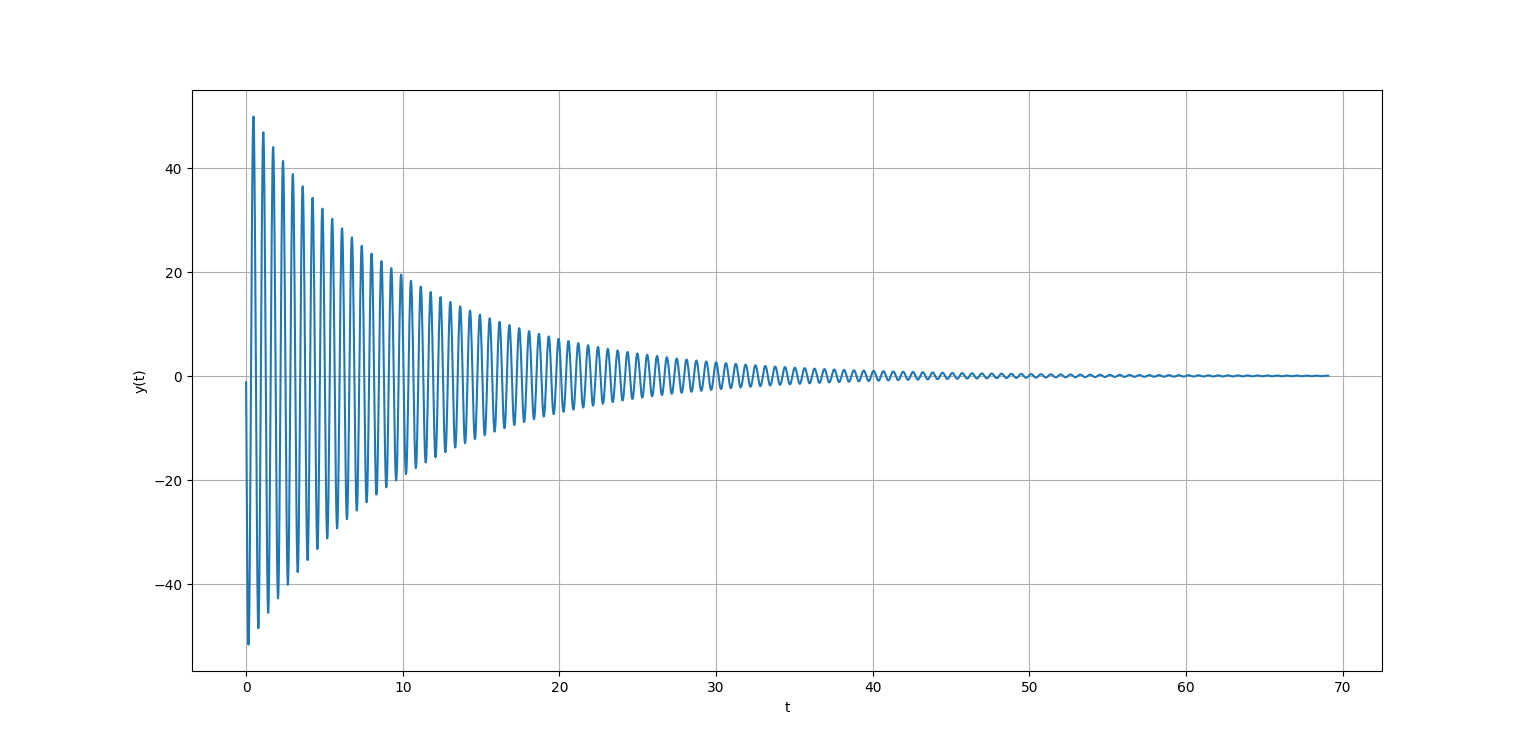
\includegraphics[scale=0.4]{impulso.png}
    \caption{Resposta ao impulso}
\end{figure}

\begin{lstlisting}
import numpy as np
import matplotlib.pyplot as plt
import control as ctrl

# 1. Definir a funcao de transferencia do sistema
num = [100, 0, 1600]  # numerador da funcao de transferencia
den = [16, 3.2, 1600]  # denominador da funcao de transferencia
sys = ctrl.TransferFunction(num, den)  # criar o objeto que representa o sistema

# 2. Calcular a resposta ao impulso
t, h = ctrl.impulse_response(sys)

# 3. Plotar do grafico da resposta ao impulso
plt.plot(t, h)
plt.xlabel('t(s)')
plt.ylabel('y(t)')
plt.grid()
plt.show()
\end{lstlisting}

\quad Observar o gráfico de resposta ao impulso de um sistema é importante porque ele fornece informações sobre como o sistema responde a um impulso de entrada.
No exemplo do trabalho, é possível perceber que a resposta ao impulso, é uma senoíde exponencialmente amortecida.

\quad Por meio da tabela, foi calculado o Laplace do cosseno de frequência $omega$ multiplicado pelo degrau unitário:

\begin{equation}
    U(s) = \mathcal{L}\{ \cos(\omega t) 1(t) \} = \frac{s}{s^2 + \omega^2}
\end{equation}

\quad Calculando o Laplace da saída do sistema sem substituir o $\omega$ da fórmula acima:

\begin{equation}
    Y(s) = H(s)U(s) = \frac{100}{16} \frac{s^2 + 16}{s^2 + 0.2s + 100} \frac{s}{s^2 + \omega^2} = \frac{100}{16} \left[ \frac{k_1s + k_2}{s^2 + 0.2s + 100} + \frac{k_3s + k_4}{s^2 + \omega^2} \right] 
\end{equation}

\begin{equation}
    s^3 + 16s = k_1s^3 + k_2s^2 + k_1\omega^2 s + k_2\omega^2 + k_3s^3 + 0.2k_3s^2 + 100k_3s + k_4s^2 + 0.2k_4s + 100k_4
\end{equation}

\begin{equation}
    \left\{
    \begin{array}{l}
        k_1 + k_3 = 1 \\
        k_2 + 0.2k_3 +k_4 = 0 \\
        \omega^2k_1 + 100k_3 + 0.2k_4 = 16 \\
        \omega^2k_2 + 100k_4 = 0
    \end{array}
    \right. 
\end{equation}

\quad Foi feito isso para que não seja necessário repetir procedimentos no desenvolvimento do trabalho.

\newpage

\section{Desenvolvimento}

\quad 1. Foi considerado uma entrada $u(t) = cos(t) 1(t)$. Foi obtido a $y(t)$ por simulação numérica utilizando Python
e as bibliotecas NumPy, Matplotlib e Control.

\begin{figure}[h]
    \centering
    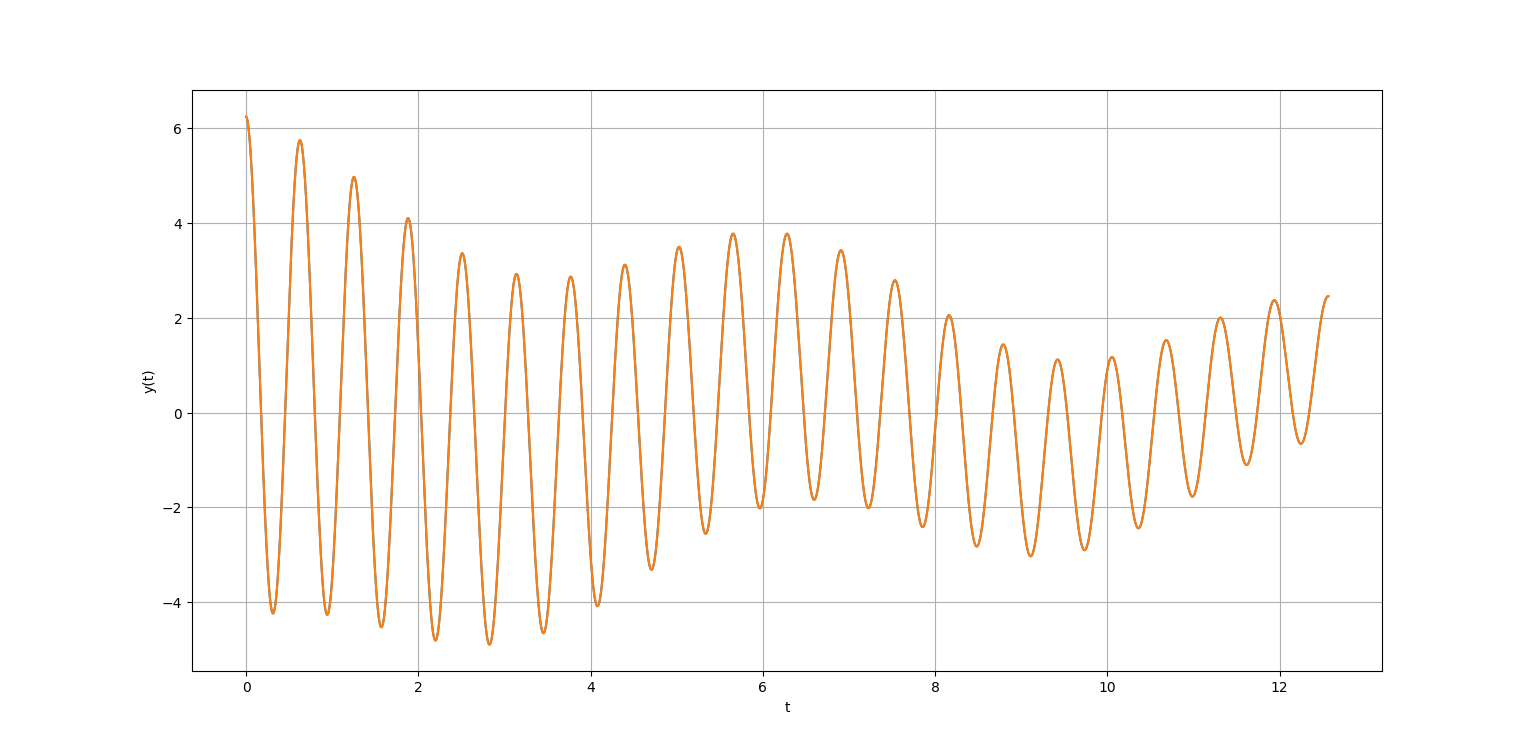
\includegraphics[scale=0.45]{questao1.png}
    \caption{Resposta ao cosseno com frequência 1 multiplicado pelo degrau unitario}
\end{figure}

\begin{lstlisting}
import numpy as np
import control as ctrl
import matplotlib.pyplot as plt

# 1. Definir a funcao de transferencia do sistema
num = [100, 0, 1600]  # numerador da funcao de transferencia
den = [16, 3.2, 1600]  # denominador da funcao de transferencia
sys = ctrl.TransferFunction(num, den)  # criar o objeto que representa o sistema

# 2. Definir os valores de tempo para simulacao
t = np.linspace(0, 4*np.pi, 10000)  # valores de tempo de 0 a 4*pi segundos

# 3. Definir o sinal de entrada como o cosseno multiplicado pelo degrau unitario
u = np.heaviside(t, 1) * np.cos(t)

# 4. Realizar a simulacao da resposta do sistema usando a funcao `control.forced_response()`
t_out, yout= ctrl.forced_response(sys, T=t, U=u)

# 5. Plotar o grafico da resposta
plt.plot(t_out, yout)
plt.xlabel('t')
plt.ylabel('y(t)')
plt.show()
\end{lstlisting}

\quad Solução analítica:

\newpage

\quad 2. Foi considerado uma entrada $u(t) = cos(4 t) 1(t)$ (frequência de zero). Foi obtido a resposta $y(t)$ por simulação numérica utilizando Python
e as bibliotecas NumPy, Matplotlib e Control.

\begin{figure}[h]
    \centering
    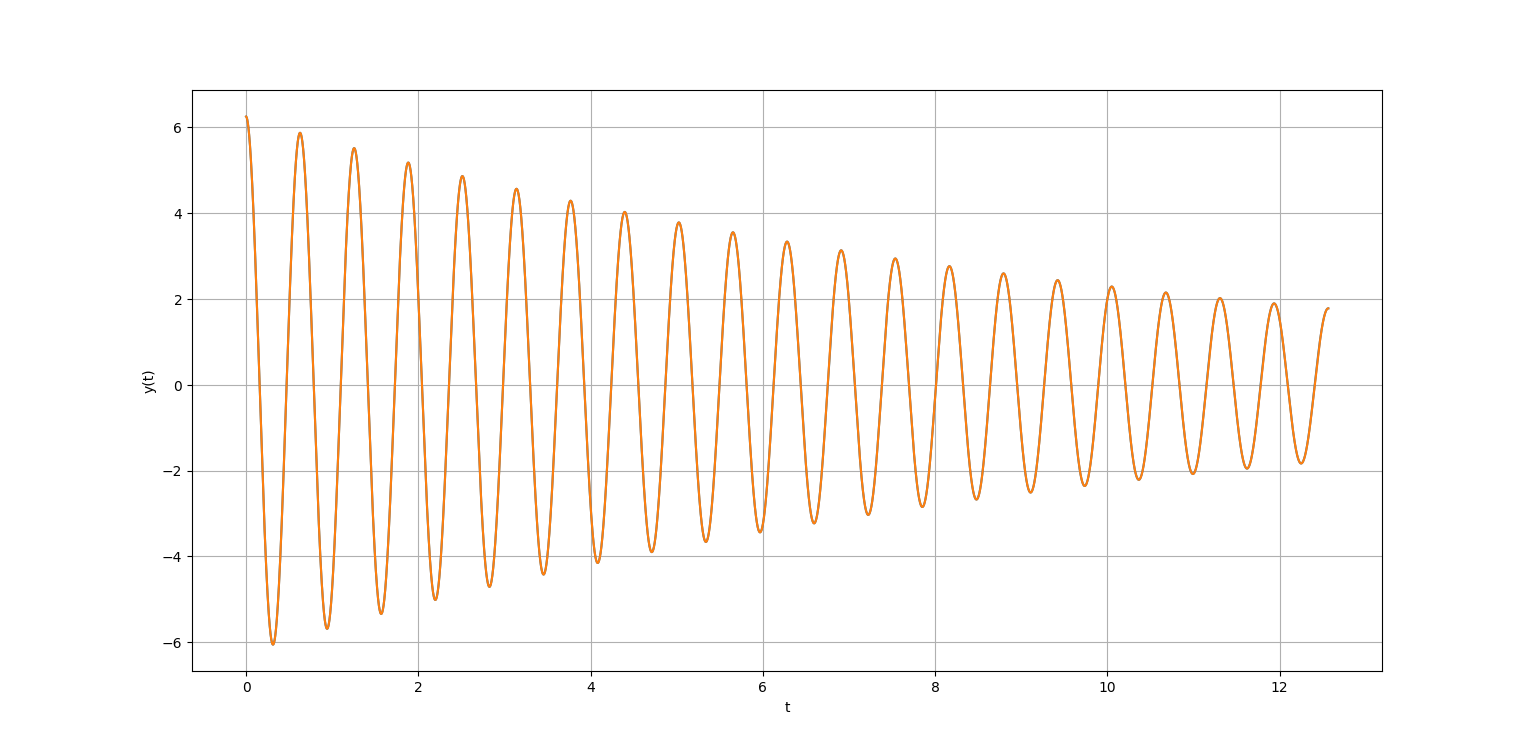
\includegraphics[scale=0.45]{questao2.png}
    \caption{Resposta ao cosseno com frequência 4 multiplicado pelo degrau unitario}
\end{figure}


\begin{lstlisting}
import numpy as np
import control as ctrl
import matplotlib.pyplot as plt

# 1. Definir a funcao de transferencia do sistema
num = [100, 0, 1600]  # numerador da funcao de transferencia
den = [16, 3.2, 1600]  # denominador da funcao de transferencia
sys = ctrl.TransferFunction(num, den)  # criar o objeto que representa o sistema

# 2. Definir os valores de tempo para simulacao
t = np.linspace(0, 4*np.pi, 10000)  # valores de tempo de 0 a 4*pi segundos

# 3. Definir o sinal de entrada como o cosseno multiplicado pelo degrau unitario
u = np.heaviside(t, 1) * np.cos(4*t)

# 4. Realizar a simulacao da resposta do sistema usando a funcao `control.forced_response()`
t_out, yout= ctrl.forced_response(sys, T=t, U=u)

# 5. Plotar o grafico da resposta
plt.plot(t_out, yout)
plt.xlabel('t')
plt.ylabel('y(t)')
plt.show()
\end{lstlisting}

\quad Solução analítica:

\newpage

\quad 3. Foi considerado uma entrada $u(t) = cos(10 t) 1(t)$. Foi obtido a resposta $y(t)$ por simulação numérica utilizando Python
e as bibliotecas NumPy, Matplotlib e Control.

\begin{figure}[h]
    \centering
    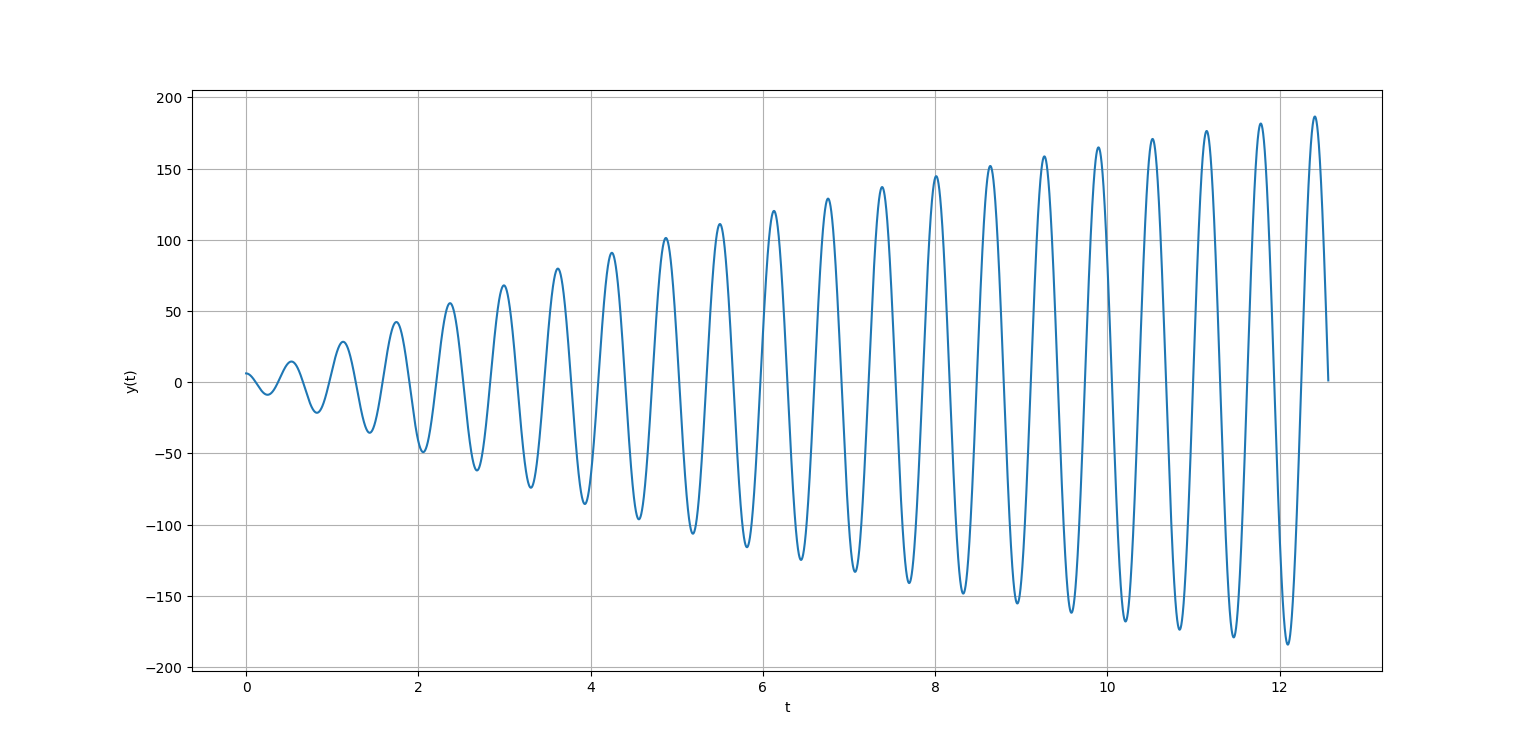
\includegraphics[scale=0.45]{questao3.png}
    \caption{Resposta ao cosseno com frequência 10 multiplicado pelo degrau unitario}
\end{figure}

\begin{lstlisting}
import numpy as np
import control as ctrl
import matplotlib.pyplot as plt

# 1. Definir a funcao de transferencia do sistema
num = [100, 0, 1600]  # numerador da funcao de transferencia
den = [16, 3.2, 1600]  # denominador da funcao de transferencia
sys = ctrl.TransferFunction(num, den)  # criar o objeto que representa o sistema

# 2. Definir os valores de tempo para simulacao
t = np.linspace(0, 4*np.pi, 10000)  # valores de tempo de 0 a 4*pi segundos

# 3. Definir o sinal de entrada como o cosseno multiplicado pelo degrau unitario
u = np.heaviside(t, 1) * np.cos(10*t)

# 4. Realizar a simulacao da resposta do sistema usando a funcao `control.forced_response()`
t_out, yout= ctrl.forced_response(sys, T=t, U=u)

# 5. Plotar o grafico da resposta
plt.plot(t_out, yout)
plt.xlabel('t')
plt.ylabel('y(t)')
plt.show()
\end{lstlisting}

\quad Solução analítica:

\newpage

\quad 4. Foi considerado uma entrada $u(t) = cos(100 t) 1(t)$. Foi obtido a resposta $y(t)$ por simulação numérica utilizando Python
e as bibliotecas NumPy, Matplotlib e Control.

\begin{figure}[h]
    \centering
    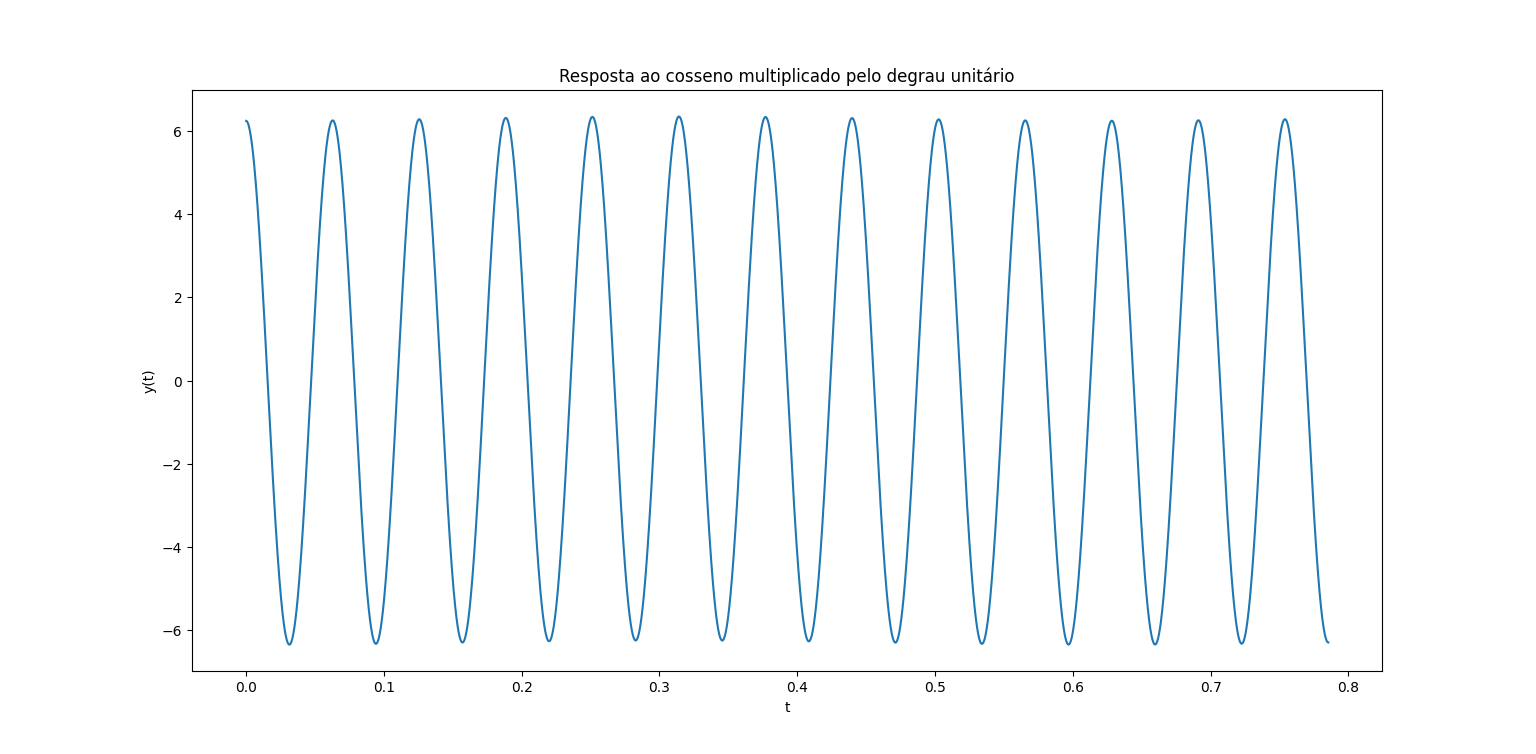
\includegraphics[scale=0.45]{questao4.png}
    \caption{Resposta ao cosseno com frequência multiplicado pelo degrau unitario}
\end{figure}

\begin{lstlisting}
import numpy as np
import control as ctrl
import matplotlib.pyplot as plt

# 1. Definir a funcao de transferencia do sistema
num = [100, 0, 1600]  # numerador da funcao de transferencia
den = [16, 3.2, 1600]  # denominador da funcao de transferencia
sys = ctrl.TransferFunction(num, den)  # criar o objeto que representa o sistema

# 2. Definir os valores de tempo para simulacao
t = np.linspace(0, 4*np.pi, 10000)  # valores de tempo de 0 a 4*pi segundos

# 3. Definir o sinal de entrada como o cosseno multiplicado pelo degrau unitario
u = np.heaviside(t, 1) * np.cos(100*t)

# 4. Realizar a simulacao da resposta do sistema usando a funcao `control.forced_response()`
t_out, yout = ctrl.forced_response(sys, T=t, U=u)

# 5. Plotar o grafico da resposta
plt.plot(t_out, yout)
plt.xlabel('t')
plt.ylabel('y(t)')
plt.show()
\end{lstlisting}

Solução analítica:

\newpage

\section{Conclusão}

\quad A resposta de um sistema linear é afetada pela localização de seus pólos e zeros.
Os pólos determinam a estabilidade e a forma como o sistema responde às diferentes entradas.
Em geral, se o sistema tem pólos na parte direita do plano complexo (parte real positiva), o sistema é instável e não pode ser utilizado em aplicações práticas.

\quad Por outro lado, se os pólos estão na parte esquerda do plano complexo (parte real negativa), o sistema é estável e pode ser usado em aplicações práticas.
A localização dos pólos também afeta a rapidez com que o sistema responde a uma entrada.
Quanto mais longe os pólos estiverem do eixo imaginário, mais rápido será a resposta do sistema.

\quad Os zeros, por outro lado, afetam a forma como o sistema responde a diferentes frequências de entrada.
Um zero em uma frequência específica anula a resposta do sistema a essa frequência,
enquanto um zero próximo a uma frequência específica pode reduzir a amplitude da resposta do sistema a essa frequência.

\newpage

\section{Extras}

\quad Plotando o Diagrama de Nyquist em Python com o seguinte código (Feito por curiosidade):

\begin{figure}[h]
    \centering
    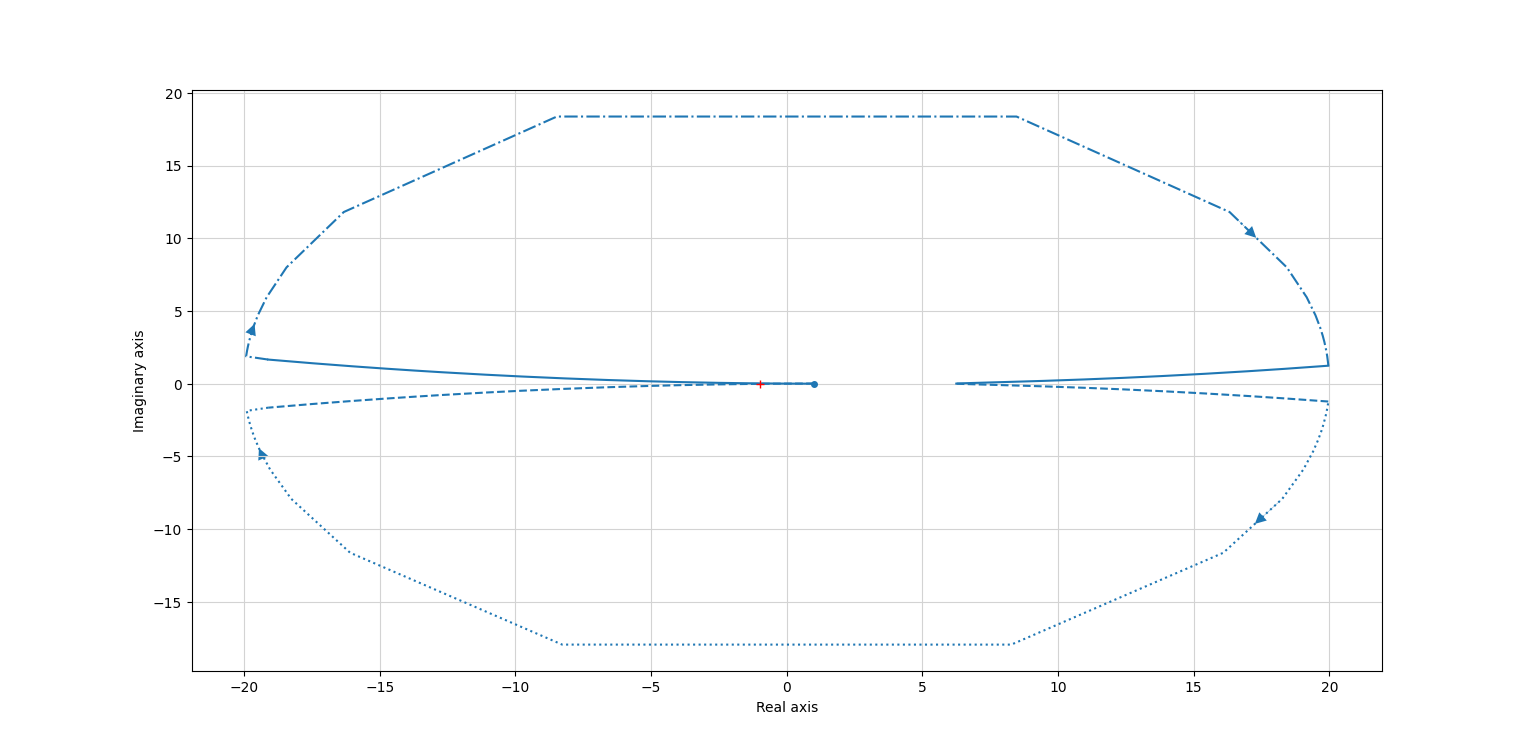
\includegraphics[scale=0.45]{nyquist.png}
    \caption{Diagrama de Nyquist}
\end{figure}

\begin{lstlisting}
import control as ctrl
import matplotlib.pyplot as plt

# 1. Definir a funcao de transferencia do sistema
num = [100, 0, 1600]  # numerador da funcao de transferencia
den = [16, 3.2, 1600]  # denominador da funcao de transferencia
H = ctrl.TransferFunction(num, den)

# 2. Plotar o diagrama de Nyquist
ctrl.nyquist_plot(H)
plt.show()
\end{lstlisting}

\end{document}